\documentclass[english]{tktltiki}
\usepackage[pdftex]{graphicx}
\usepackage{subfigure}
\usepackage{url}
\begin{document}
%\doublespacing
%\singlespacing
\onehalfspacing

\title{Digital Humanities Hackathon 2017 in Helsinki  \\ 
	Experiences by a computer scientist}
\author{P�ter Ivanics}
\date{\today}

\maketitle

\numberofpagesinformation{\numberofpages\ pages + \numberofappendixpages\ appendices}

% \mytableofcontents

\section{Introduction}
	Digital humanities is an emerging field of science, which applies modern data processing methods to answer social science and humanities oriented research questions. This way scholars can study their own field from a new angle via the application of methods traditionally used in computer science. As a result, humanist researchers do not necessarily have to closely read historical text, but can take a look at the data from a new point of view, from a different angle. As the amount of such text has grown large along the centuries, manual labour has proven not to be sufficient to process all of the material and there is need for the assistance of computational methods. 
	
	I was lucky enough to participate in the Digital Humanities Hackathon organized by University of Helsinki and Aalto University in this year. During an intensive week of collaboration May 2017, historians, linguists, psychologists and computer scientists were brought together under the hood of this event.	 This report shortly summarizes my own experiences as a member of one of the interdisciplinary groups working on the digitized archive of Finnish newspapers from the 19th century. 
	
\section{Why should computer scientists join events like this?}
	There are various events why I joined this event. First of all, as someone living abroad for over 3 years, I worked together with many people from different backgrounds and nations. Every single time I worked with somebody from a previously unseen cultural or professional background, I learned or experienced something new. Collaboration with people outside of my own interests and culture always opens my eyes that things can be done and looked at differently. 
	
	I have never worked with anyone with background in humanistic sciences, language studies or history, and therefore I considered this as a superb opportunity. From the very first moment I knew, one of the challenges will be to be on the same page and understand how a to bring computer science terms and working methods under this umbrella. 
	
	Last, but not least I believe this hackathon was something unique in nature, which does not happen every weekend. The preliminary topics and problem descriptions were stimulating, generally research-oriented, which is typically not the case on hackathons. I was not totally sure what to expect or how sufficient my skills are going to be, but more enthusiastic than ever to get started working on the given problems. 

\section{What did we do?}
	The group \textit{Categories, norms and genres - critical reading in numbers} consisted of two historians, two computer scientists, two linguists and a philosopher. On top of that, the composition of the group was not only interdisciplinary but also intercultural, because members were coming from four different countries. 
	
	The team was given access to the Digital Newspaper Archive, which contains huge amount of digitized material from newspapers and journals published in Finland. Some of the data is freely available for anybody to process, but a considerable amount is copyrighted (Figure \ref{data_in_digi}). 
	
	\begin{figure}[h] 
		\begin{center}
			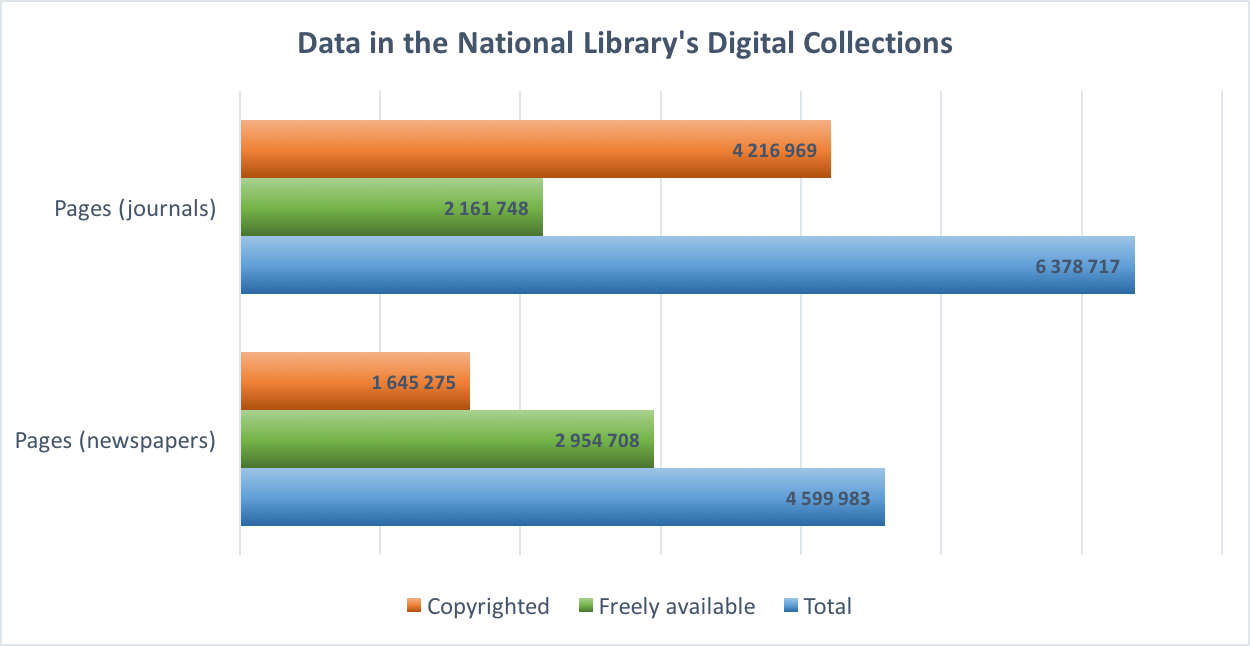
\includegraphics[width=0.9\textwidth]{images/data_in_digi.png}
			\caption{The distribution of the data in the digital archive of the Finnish National Library.}
			\label{data_in_digi}
		\end{center}
	\end{figure}	
	
	During the three orientation days, our team discussed to aim for genre detection in the given corpus. As this scope was too wide in general, we decided to scale down the aims for poetry detection via computational methods. I came to the understanding that social sciences do not typically utilize computational methods or even know about the capabilities of modern Data Mining and Machine Learning techniques, which was a bit of a shock to me. Similarly I realized, that my understanding on humanistic terms, such as corpus, genre, literary history or topic modeling requires some refreshment. 
	
	Despite the fact I study computer science, my skills are not extremely developed in this field, which was a bit of a concern in the beginning. However, we made a good combination with my fellow team mate with similar background, as he had hands-on experience with Machine Learning methods, while I could communicate with everybody in the team. I was able to explain the basic ideas and capabilities of the field of Machine Learning to humanists and point out the directions our team should aim for, which was very much appreciated. This was mainly based on the SKLearn framework and the text analysis tutorial provided online.
	
	We spent significant amount of time during development phase of the project with pair programming the algorithm and finding out which approach suits our case the best. In the end we have chosen a Support Vector Machine with relative word frequency analysis as features. We put together the parser logic in a day and the algorithm the next day, however there were many iterations with the humanist team mates to evaluate and improve on the accuracy. The performance on the test data of around 50 \% was greatly improved by the presentation day and it was awesome to see how much progress we made in such a short time. 

	I see my role as a connective person in this team between computer science and the rest of the team rather than a programmer. Nevertheless, I did some coding during the hackathon, which meant actively reviewing and contributing to the ML algorithm written in Python and creating some visualization scripts on the output data in R (outcome listed in the bottom of this post). For a short while, I did some technical support also to the humanists in our team, as they liked the way I explained what our scripts do and how data visualization is done. On top of that, this was a great opportunity to refresh and further develop my experiences in R scripting, Python development and public speaking via the final presentation. 
	
	All of our code is freely available in the GitHub repository listed in the references. During the last two day of the event, I contributed to the content of our poster and prepared material for the presentation, where I was given the role of presenting the technical background and results of our team. 

\section{Conclusions}
	In many cases we had to exchange thoughts on the team level to ensure everybody understands the reasons why something is (not) needed, (not) relevant or (not) possible. It was very interesting to see how the two fields of science can cooperate successfully. Communication was proven to be a key in this project and I can say our team did this in the best possible way. We gave eachother room to explain the goals and the obstacles on a required level so we stay on the same page. 
	
	For me this hackathon was a great example on how interdisciplinary teams can corporate and how much communication matters in such situations. As the "mentors" (teachers) of the team were organizing the tasks and kept everybody engaged during the whole week, nobody was left alone in their work. Communication was very well established at the first place and therefore was fluent all the way. 

	As a conclusion, it was an amazing experience to participate in a hackathon like this. I strongly encourage all programmers to be open for cooperation from outside of our own industry. Hackathons like this are superb opportunities also to find out new workflows, to learn about new things, to meet new people and to have some fun with people, who you may never do otherwise. 
	
\lastpage

\appendices

\pagestyle{empty}

\internalappendix{1}{Links}
	\begin{enumerate}
		\item Digital Newspaper Archive: \url{http://digi.kansalliskirjasto.fi/?language=en}
		\item Scikit learn - Working With Text Data \url{http://scikit-learn.org/stable/tutorial/text_analytics/working_with_text_data.html}
		\item GitHub repository: \url{https://github.com/dhh17/categories_norms_genres}
		\item Google drive folder: \url{https://drive.google.com/open?id=0B3BOLzrUa2EaeVlkRHJtNU00eVk}
	\end{enumerate}

\internalappendix{2}{Charts}
		\begin{center}
			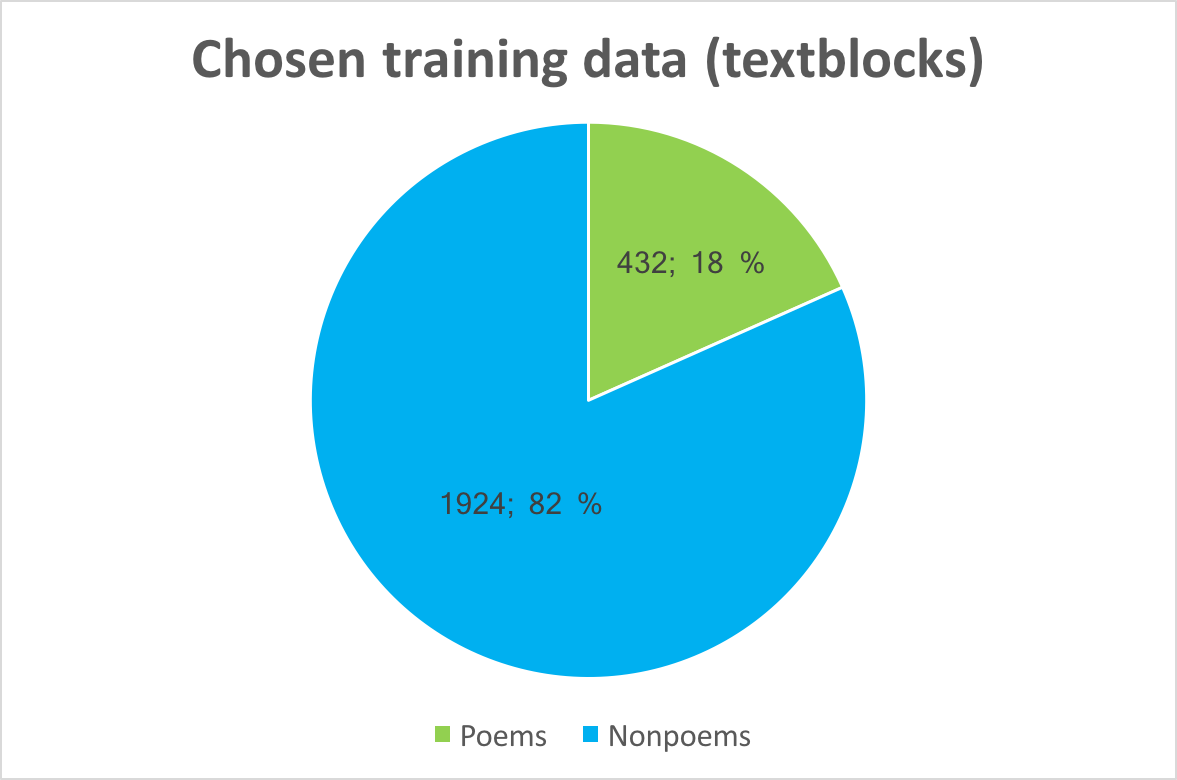
\includegraphics[width=0.9\textwidth]{images/training_data_distribution.png} \\
			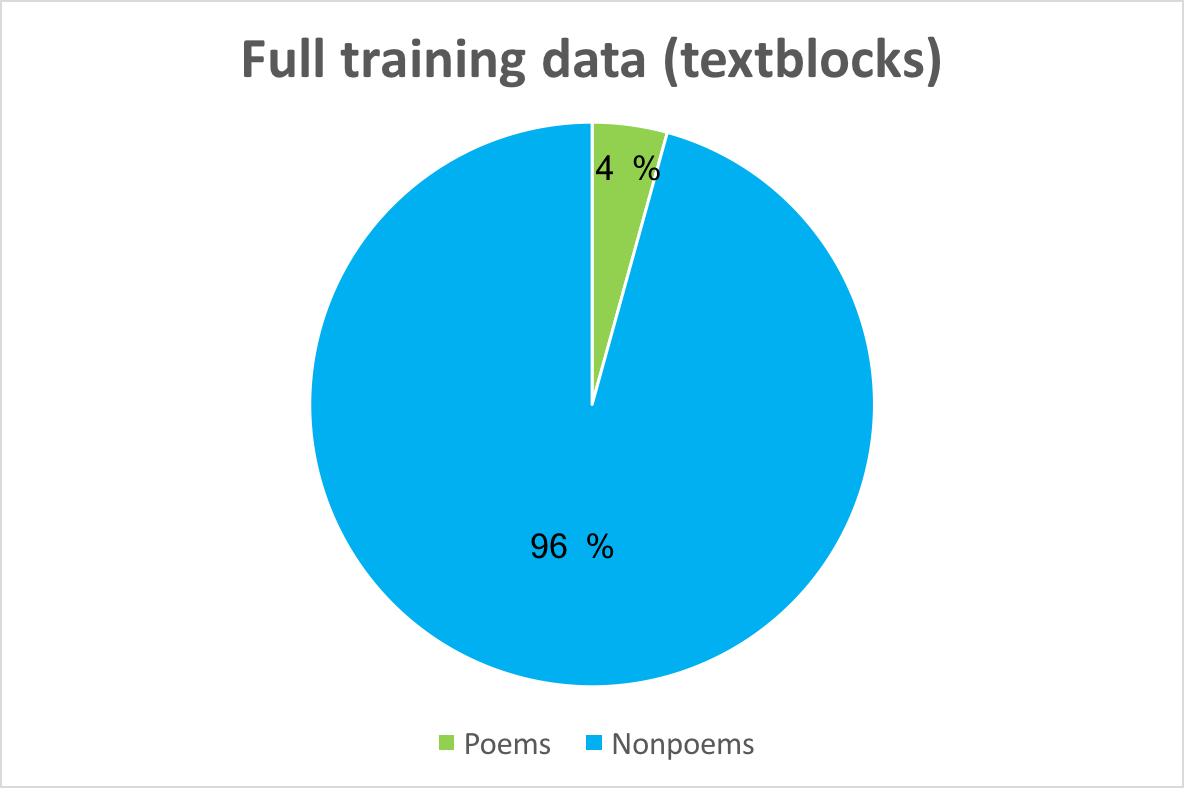
\includegraphics[width=0.9\textwidth]{images/full_training_data.png} \\
			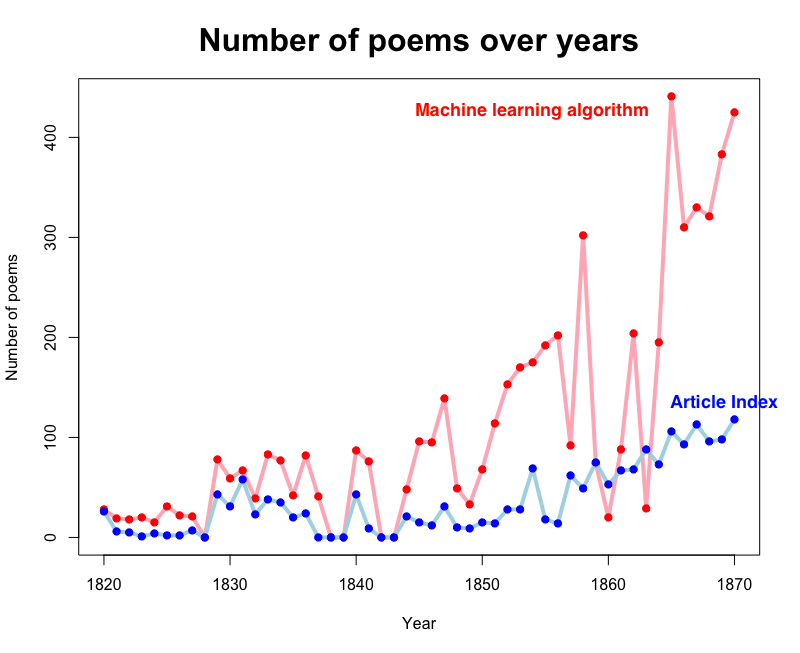
\includegraphics[width=0.9\textwidth]{images/number_of_poems_by_year.png} \\
			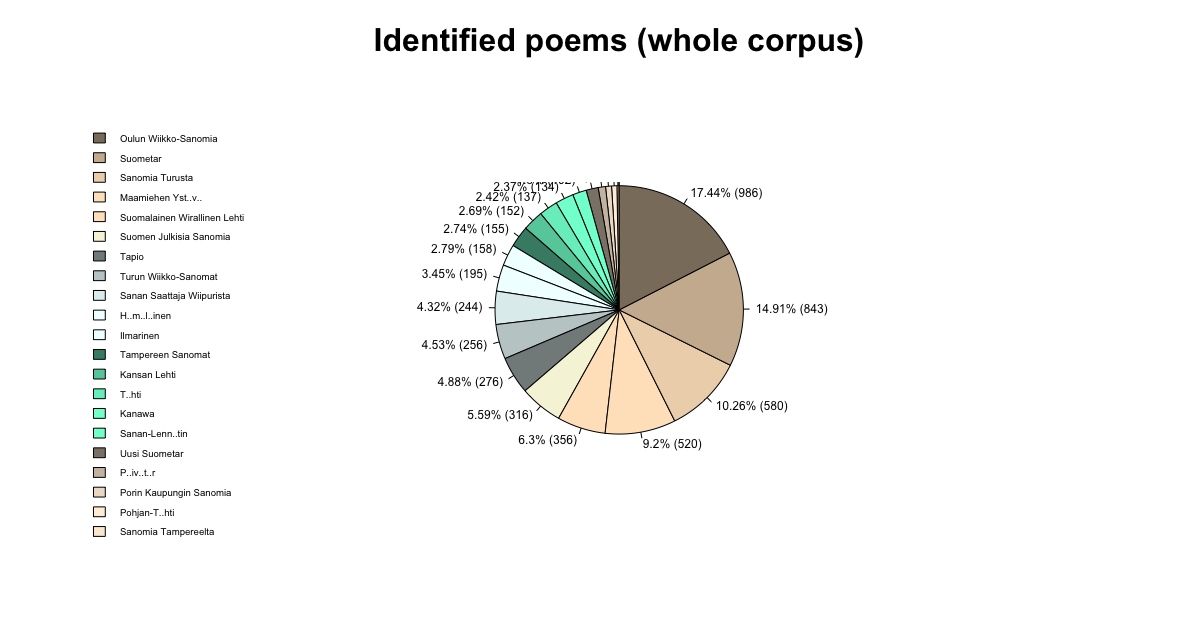
\includegraphics[width=0.9\textwidth]{images/pie_chart_of_identified_poems.png} \\
			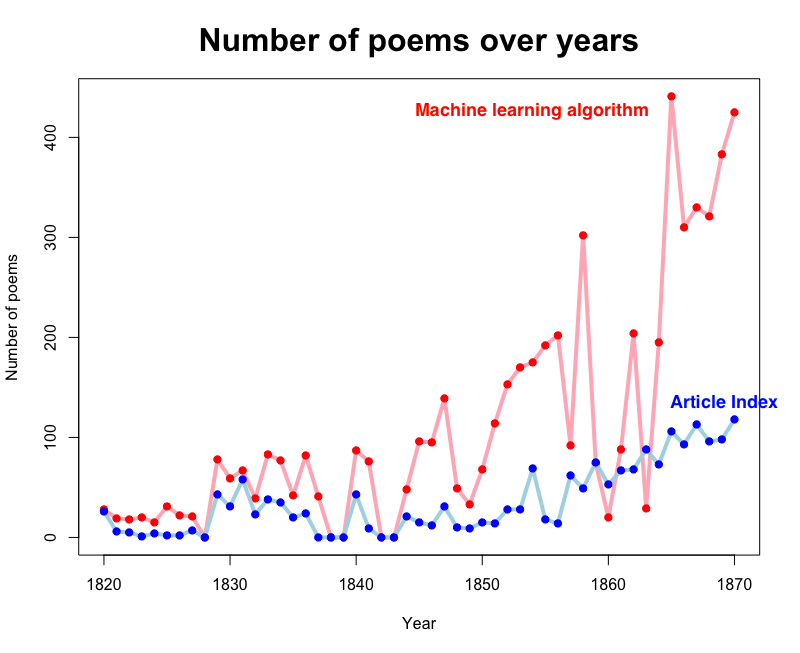
\includegraphics[width=0.9\textwidth]{images/number_of_poems_by_year.png}
		\end{center}
\end{document}